\documentclass[11pt]{article}
\usepackage[letterpaper, left=20mm, right=20mm, bottom=30mm, top=30mm]{geometry} % page margins
\usepackage{graphicx} % includegraphics

\begin{document}

\begin{figure}
    \centering
    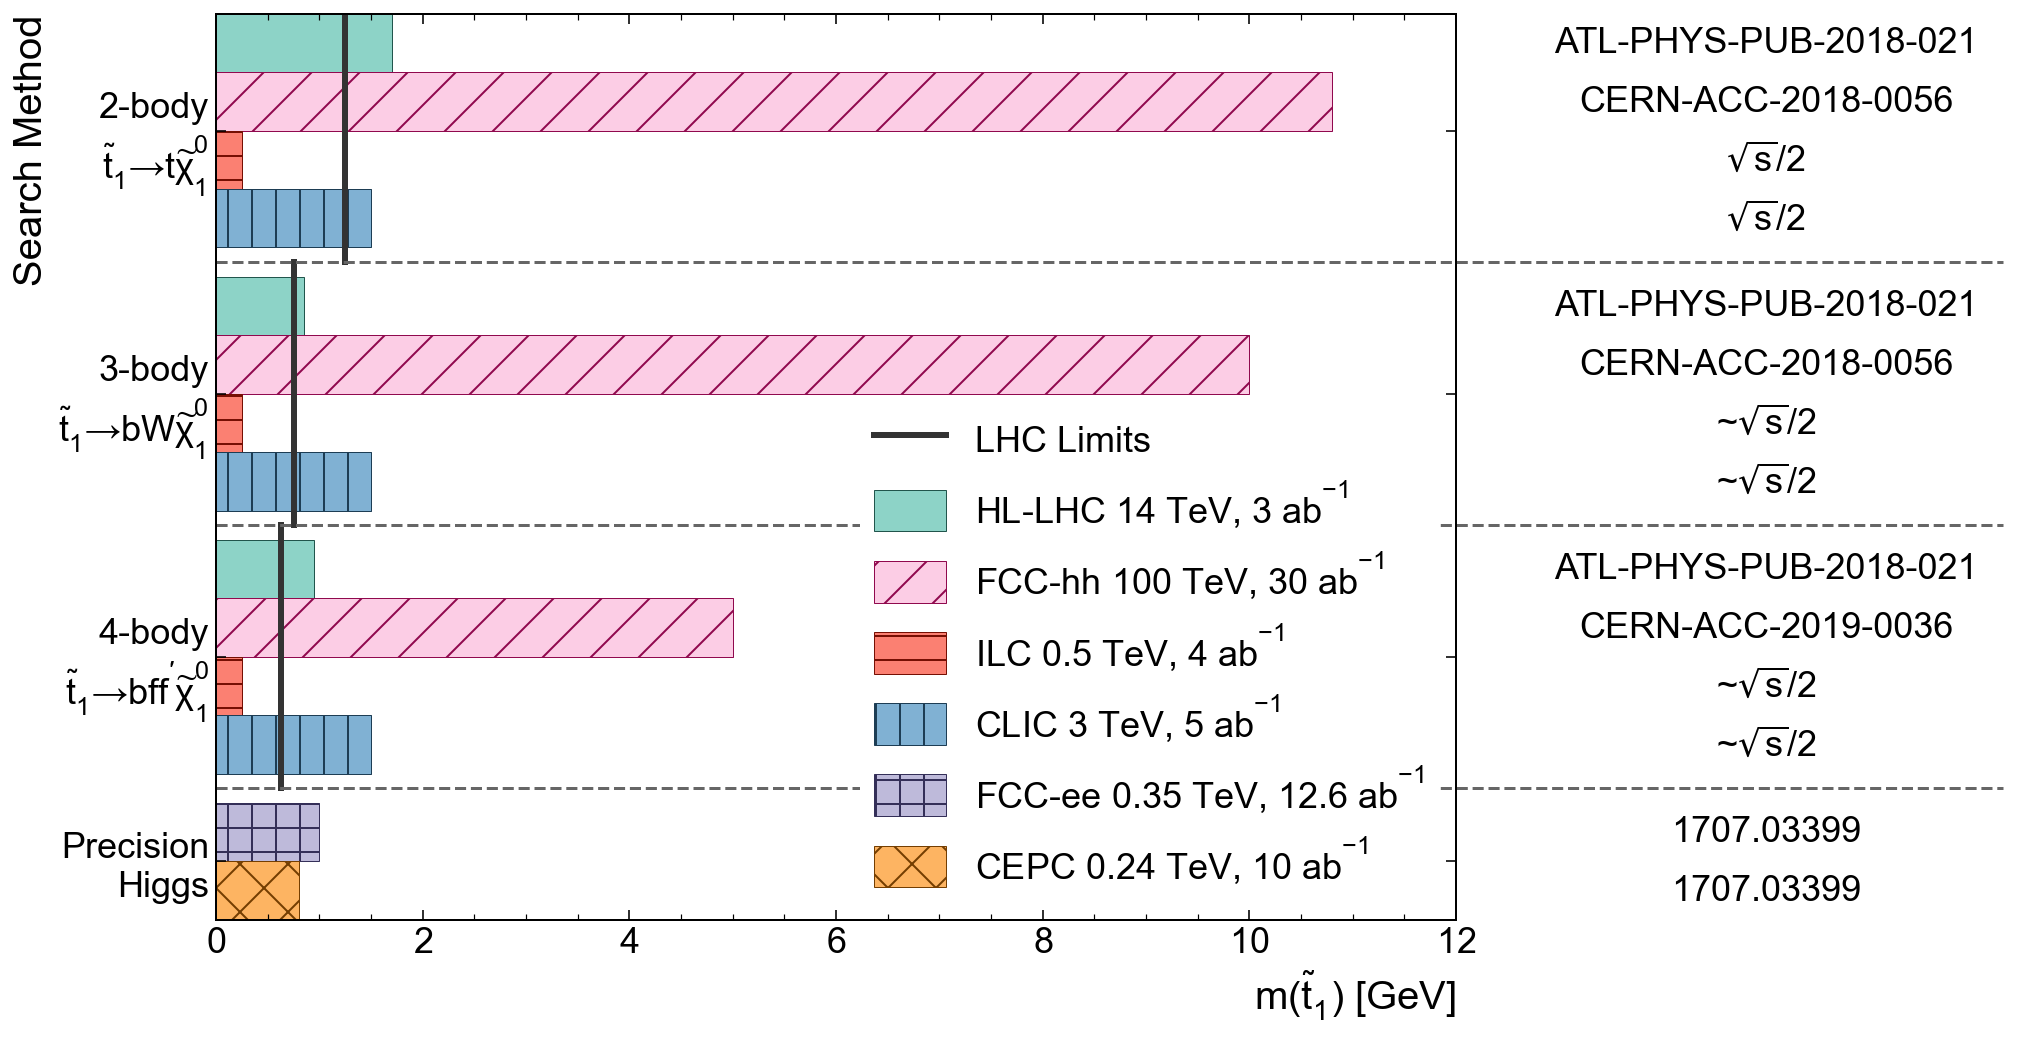
\includegraphics[width=\textwidth]{stop.png}
    \caption{Estimated stop exculsion reaches for various colliders and search methods. 
    The two, three, and four-body decay searches target the regions $\Delta m(\widetilde{t}_1, \widetilde{\chi}_1^0) \in (m_t, \infty)$, $(m_b + m_W, m_t)$, and $(0, m_b + m_W)$ respectively. 
    The bars show the largest limit on $m(\widetilde{t}_1)$ in the $m(\widetilde{t}_1)-m(\widetilde{\chi}_1^0)$ phase-space for each region. 
    The Precision Higgs constraints are based on measuring production rates of the Higgs boson assuming the only BSM contributions are from stops. 
    References for each exclusion estimate are shown on the right as either the CDS report number or arXiv identifier. 
    ILC and CLIC limits are estimated to be $\sqrt{s}/2$, with slight inefficiencies in the three and four-body decay searches due to soft decay products. Current limits from the LHC \cite{ATL-PHYS-PUB-2022-013} are shown as vertical lines. }
\end{figure}



\end{document}
